%!TEX TS-program = xelatex
\documentclass[11pt]{article}

\usepackage[english]{babel}

\usepackage{amsmath,amssymb,amsfonts}
\usepackage[utf8]{inputenc}
\usepackage[T1]{fontenc}
\usepackage{stix2}
\usepackage[scaled]{helvet}
\usepackage[scaled]{inconsolata}

\usepackage{lastpage}

\usepackage{gensymb}

\usepackage{setspace}

\usepackage{ccicons}

\usepackage[hang,flushmargin]{footmisc}

\usepackage{geometry}

\setlength{\parindent}{0pt}
\setlength{\parskip}{6pt plus 2pt minus 1pt}

\usepackage{fancyhdr}
\renewcommand{\headrulewidth}{0pt}\providecommand{\tightlist}{%
  \setlength{\itemsep}{0pt}\setlength{\parskip}{0pt}}

\makeatletter
\newcounter{tableno}
\newenvironment{tablenos:no-prefix-table-caption}{
  \caption@ifcompatibility{}{
    \let\oldthetable\thetable
    \let\oldtheHtable\theHtable
    \renewcommand{\thetable}{tableno:\thetableno}
    \renewcommand{\theHtable}{tableno:\thetableno}
    \stepcounter{tableno}
    \captionsetup{labelformat=empty}
  }
}{
  \caption@ifcompatibility{}{
    \captionsetup{labelformat=default}
    \let\thetable\oldthetable
    \let\theHtable\oldtheHtable
    \addtocounter{table}{-1}
  }
}
\makeatother

\usepackage{array}
\newcommand{\PreserveBackslash}[1]{\let\temp=\\#1\let\\=\temp}
\let\PBS=\PreserveBackslash

\usepackage[breaklinks=true]{hyperref}
\hypersetup{colorlinks,%
citecolor=blue,%
filecolor=blue,%
linkcolor=blue,%
urlcolor=blue}
\usepackage{url}

\usepackage{caption}
\setcounter{secnumdepth}{0}
\usepackage{cleveref}

\usepackage{graphicx}
\makeatletter
\def\maxwidth{\ifdim\Gin@nat@width>\linewidth\linewidth
\else\Gin@nat@width\fi}
\makeatother
\let\Oldincludegraphics\includegraphics
\renewcommand{\includegraphics}[1]{\Oldincludegraphics[width=\maxwidth]{#1}}

\usepackage{longtable}
\usepackage{booktabs}

\usepackage{color}
\usepackage{fancyvrb}
\newcommand{\VerbBar}{|}
\newcommand{\VERB}{\Verb[commandchars=\\\{\}]}
\DefineVerbatimEnvironment{Highlighting}{Verbatim}{commandchars=\\\{\}}
% Add ',fontsize=\small' for more characters per line
\usepackage{framed}
\definecolor{shadecolor}{RGB}{248,248,248}
\newenvironment{Shaded}{\begin{snugshade}}{\end{snugshade}}
\newcommand{\KeywordTok}[1]{\textcolor[rgb]{0.13,0.29,0.53}{\textbf{#1}}}
\newcommand{\DataTypeTok}[1]{\textcolor[rgb]{0.13,0.29,0.53}{#1}}
\newcommand{\DecValTok}[1]{\textcolor[rgb]{0.00,0.00,0.81}{#1}}
\newcommand{\BaseNTok}[1]{\textcolor[rgb]{0.00,0.00,0.81}{#1}}
\newcommand{\FloatTok}[1]{\textcolor[rgb]{0.00,0.00,0.81}{#1}}
\newcommand{\ConstantTok}[1]{\textcolor[rgb]{0.00,0.00,0.00}{#1}}
\newcommand{\CharTok}[1]{\textcolor[rgb]{0.31,0.60,0.02}{#1}}
\newcommand{\SpecialCharTok}[1]{\textcolor[rgb]{0.00,0.00,0.00}{#1}}
\newcommand{\StringTok}[1]{\textcolor[rgb]{0.31,0.60,0.02}{#1}}
\newcommand{\VerbatimStringTok}[1]{\textcolor[rgb]{0.31,0.60,0.02}{#1}}
\newcommand{\SpecialStringTok}[1]{\textcolor[rgb]{0.31,0.60,0.02}{#1}}
\newcommand{\ImportTok}[1]{#1}
\newcommand{\CommentTok}[1]{\textcolor[rgb]{0.56,0.35,0.01}{\textit{#1}}}
\newcommand{\DocumentationTok}[1]{\textcolor[rgb]{0.56,0.35,0.01}{\textbf{\textit{#1}}}}
\newcommand{\AnnotationTok}[1]{\textcolor[rgb]{0.56,0.35,0.01}{\textbf{\textit{#1}}}}
\newcommand{\CommentVarTok}[1]{\textcolor[rgb]{0.56,0.35,0.01}{\textbf{\textit{#1}}}}
\newcommand{\OtherTok}[1]{\textcolor[rgb]{0.56,0.35,0.01}{#1}}
\newcommand{\FunctionTok}[1]{\textcolor[rgb]{0.00,0.00,0.00}{#1}}
\newcommand{\VariableTok}[1]{\textcolor[rgb]{0.00,0.00,0.00}{#1}}
\newcommand{\ControlFlowTok}[1]{\textcolor[rgb]{0.13,0.29,0.53}{\textbf{#1}}}
\newcommand{\OperatorTok}[1]{\textcolor[rgb]{0.81,0.36,0.00}{\textbf{#1}}}
\newcommand{\BuiltInTok}[1]{#1}
\newcommand{\ExtensionTok}[1]{#1}
\newcommand{\PreprocessorTok}[1]{\textcolor[rgb]{0.56,0.35,0.01}{\textit{#1}}}
\newcommand{\AttributeTok}[1]{\textcolor[rgb]{0.77,0.63,0.00}{#1}}
\newcommand{\RegionMarkerTok}[1]{#1}
\newcommand{\InformationTok}[1]{\textcolor[rgb]{0.56,0.35,0.01}{\textbf{\textit{#1}}}}
\newcommand{\WarningTok}[1]{\textcolor[rgb]{0.56,0.35,0.01}{\textbf{\textit{#1}}}}
\newcommand{\AlertTok}[1]{\textcolor[rgb]{0.94,0.16,0.16}{#1}}
\newcommand{\ErrorTok}[1]{\textcolor[rgb]{0.64,0.00,0.00}{\textbf{#1}}}
\newcommand{\NormalTok}[1]{#1}

\newlength{\cslhangindent}
\setlength{\cslhangindent}{1.5em}
\newlength{\csllabelwidth}
\setlength{\csllabelwidth}{3em}
\newenvironment{CSLReferences}[2] % #1 hanging-ident, #2 entry spacing
 {% don't indent paragraphs
  \setlength{\parindent}{0pt}
  % turn on hanging indent if param 1 is 1
  \ifodd #1 \everypar{\setlength{\hangindent}{\cslhangindent}}\ignorespaces\fi
  % set entry spacing
  \ifnum #2 > 0
  \setlength{\parskip}{#2\baselineskip}
  \fi
 }%
 {}
\usepackage{calc} % for \widthof, \maxof
\newcommand{\CSLBlock}[1]{#1\hfill\break}
\newcommand{\CSLLeftMargin}[1]{\parbox[t]{\maxof{\widthof{#1}}{\csllabelwidth}}{#1}}
\newcommand{\CSLRightInline}[1]{\parbox[t]{\linewidth}{#1}}
\newcommand{\CSLIndent}[1]{\hspace{\cslhangindent}#1}\geometry{verbose,letterpaper,tmargin=2.2cm,bmargin=2.2cm,lmargin=2.2cm,rmargin=2.2cm}

\usepackage{lineno}
\usepackage[nolists,noheads]{endfloat}

\pagestyle{plain}

\tolerance=1
\emergencystretch=\maxdimen
\hyphenpenalty=10000
\hbadness=10000

\doublespacing

\fancypagestyle{normal}
{
  \fancyhf{}
  \fancyfoot[R]{\footnotesize\sffamily\thepage\ of \pageref*{LastPage}}
}
\begin{document}
\raggedright
\thispagestyle{empty}
{\Large\bfseries\sffamily Template to prepare preprints and manuscripts
using markdown and github actions}
\vskip 5em

%
\href{https://orcid.org/0000-0002-0735-5184}{Timothée\,Poisot}%
%
\,\textsuperscript{1,2,‡}\quad %
Peregrin\,Took%
%
\,\textsuperscript{3,4}\quad %
Merriadoc\,Brandybuck%
%
\,\textsuperscript{4,5,‡}

\textsuperscript{1}\,Université de
Montréal\quad \textsuperscript{2}\,Québec Centre for Biodiversity
Sciences\quad \textsuperscript{3}\,Inn of the Prancing
Pony\quad \textsuperscript{4}\,Fellowship of the
Ring\quad \textsuperscript{5}\,Green Dragon Inn

\textsuperscript{‡}\,Equal contributions\\

\textbf{Correspondance to:}\\
Timothée Poisot --- \texttt{timothee.poisot@umontreal.ca}\\

\vfill



        {\bfseries Purpose:}\,This template provides a series of scripts
to render a markdown document into an interactive website and a series
of PDFs.\\%
        {\bfseries Internals:}\,GitHub actions and a series of python
scritpts. The markdown is handled with \texttt{pandoc}.\\%
        {\bfseries Motivation:}\,It makes collaborating on text with
GitHub easier, and means that we never need to think about the
output.\\%
    

\vfill
This work is released by its authors under a CC-BY 4.0 license\hfill\ccby\\
Last revision: \emph{\today}

\clearpage
\thispagestyle{empty}

\vfill

\vfill

\clearpage
\linenumbers
\pagestyle{normal}

This template uses \texttt{pandoc} (and a few additional \emph{Julia}
glue scripts) to facilitate the production of scientific articles using
a standard markdown file. The objective is to ensure that standard
markdown (with the important exception of the \texttt{pandoc-crossref}
citation markup) will be rendered into an interactive website (which
allows collaborative annotations with the \texttt{hypothes.is}
platform), a ``draft'' style PDF (double-spaced, numbered lines, figures
at the end), and a ``preprint'' style PDF (with more reader-friendly
pagination).

The core bit of configuration is the \texttt{metadata.json} file, which
handles information about authorship, affiliations, the abstract,
keywords, etc. All documents will be deployed to \texttt{gh-pages}
\emph{only} on push events from the \texttt{main} branch. All of the
artifacts will be built when doing pull requests, so you can check that
merging a branch is \emph{not} going to cause the compilation of the
documents to fail; indeed, you can download the artifacts produced
during the run, to check the PDF and html files. The website is only
updated from the \texttt{main} branch.

The workflow is \emph{very} GitHub based, and so the manuscript file
\emph{is} the \texttt{README.md} - this is not going to be a huge issue
as 90\% of the markdown is standard, with the exception of the citations
and mathematics, so this will render (mostly) like a normal README file.

\hypertarget{deploying-the-template}{%
\section{Deploying the template}\label{deploying-the-template}}

The process of deploying this template has been \emph{greatly}
streamlined from previous versions:

\begin{itemize}
\tightlist
\item
  Click on the ``Use this template'' button
\item
  Edit \texttt{README.md} with your own text, commit, and push
\item
  This push will trigger the first build - the builds are only active on
  the \texttt{main} branch (\emph{not} \texttt{master}!), and on pull
  requests
\item
  Go to \texttt{http://you.github.io/repo-name/} to view the html
  version, and get access to the PDFs
\item
  Add your references to the \texttt{references.bib} file
\item
  Edit the \texttt{metadata.json} file to add the title, abstract,
  authors
\end{itemize}

In particular, note that \emph{you do not need} to create a personnal
access token to deploy to \texttt{gh-pages} (from where the website is
served).

\hypertarget{the-metadata-file}{%
\section{The metadata file}\label{the-metadata-file}}

\hypertarget{general-information}{%
\subsection{General information}\label{general-information}}

The title is a field in the \texttt{metadata.json}:

\begin{Shaded}
\begin{Highlighting}[]
\FunctionTok{\{}
    \DataTypeTok{"title"}\FunctionTok{:} \StringTok{"Preprint template"}
\FunctionTok{\}}
\end{Highlighting}
\end{Shaded}

\hypertarget{authorship}{%
\subsection{Authorship}\label{authorship}}

Authors are listed as objects in the \texttt{authors} block. Each author
is specified as follows:

\begin{Shaded}
\begin{Highlighting}[]
\FunctionTok{\{}
      \DataTypeTok{"familyname"}\FunctionTok{:} \StringTok{"Bob"}\FunctionTok{,}
      \DataTypeTok{"givennames"}\FunctionTok{:} \StringTok{"Alice"}\FunctionTok{,}
      \DataTypeTok{"email"}\FunctionTok{:} \StringTok{"alice.bob@u.edu"}\FunctionTok{,}
      \DataTypeTok{"orcid"}\FunctionTok{:} \StringTok{"0000{-}0000{-}0000{-}0001"}\FunctionTok{,}
      \DataTypeTok{"affiliations"}\FunctionTok{:} \OtherTok{[}
        \StringTok{"Affiliation 1"}\OtherTok{,}
        \StringTok{"Affiliation 2"}
      \OtherTok{]}\FunctionTok{,}
      \DataTypeTok{"status"}\FunctionTok{:} \OtherTok{[}\StringTok{"corresponding"}\OtherTok{,} \StringTok{"equal"}\OtherTok{]}
    \FunctionTok{\}}
\end{Highlighting}
\end{Shaded}

The \texttt{email} field is recommended for all authors. The
\texttt{status} field is only useful for the corresponding author, and
to denote equal contributions. These informations are rendered on the
initial page. If an \texttt{orcid} is given, it will be linked on the
HTML and PDF versions.

Note that there is \emph{no need} to number the affiliations - a small
python script will take care of this automatically.

\hypertarget{abstract}{%
\subsection{Abstract}\label{abstract}}

This template supports three types of abstracts, indicated in the
metadata file as \texttt{abstract}:

A regular \texttt{abstract} is defined as

\begin{Shaded}
\begin{Highlighting}[]
\ErrorTok{"abstract":} \ErrorTok{"A} \ErrorTok{very} \ErrorTok{long} \ErrorTok{string"}
\end{Highlighting}
\end{Shaded}

An itemized abstract is an array of strings, each representing a bullet
point:

\begin{Shaded}
\begin{Highlighting}[]
\ErrorTok{"abstract":} \OtherTok{[}
    \StringTok{"Point 1"}\OtherTok{,}
    \StringTok{"Point 2"}
\OtherTok{]}
\end{Highlighting}
\end{Shaded}

A structured abstract is an object with key-value pairs :

\begin{Shaded}
\begin{Highlighting}[]
\ErrorTok{"abstract":} \FunctionTok{\{}
    \DataTypeTok{"Location"}\FunctionTok{:} \StringTok{"Worldwide"}\FunctionTok{,}
    \DataTypeTok{"Organisms"}\FunctionTok{:} \StringTok{"Mammals"}
\FunctionTok{\}}
\end{Highlighting}
\end{Shaded}

\hypertarget{citation-style}{%
\subsection{Citation style}\label{citation-style}}

The \texttt{citationstyle} key corresponds to the name, with
\texttt{.csl} ommited, of a CSL stylesheet stored in the
\href{https://github.com/citation-style-language/}{citation style
language} repository. Note that there is no difference between main and
dependent styles, the build engine will take the correct steps to get
the correct style. The default is
\texttt{"citationstyle":\ "ecology-letters"}. There is a longer section
about references management later on.

\hypertarget{references-management}{%
\section{References management}\label{references-management}}

The references are managed by \texttt{pandoc}. Note that we \emph{do
not} use \texttt{pandoc-citeproc}, which was an external module for
older \texttt{pandoc} versions. References \emph{must} be stored in a
\texttt{references.bib} file, and that it would make sense to order it
alphabetically by key.

We use \href{https://www.zotero.org/}{Zotero} for references management,
and for the lab's manuscripts, we work from folders in a shared library
(with a folder for every manuscript).

It is recommedned to use the
\href{https://retorque.re/zotero-better-bibtex/}{Better BibTeX} plugin
for citation key generations, and auto-export of the shared library to
the \texttt{references.bib} file. We use a citation key format meant to
convey information on the author (first author full name), date (complet
year), and title (first three letters of the first two non-stop words).
It must be set in the Better BibTeX preferences as (you might need to
remove the line changes):

\begin{verbatim}
auth.fold.fold + year + title.fold.nopunctordash.skipwords.lower.select(1,1).capitalize()
\end{verbatim}

It is a good idea to configure Better BibTeX to auto-export on change,
and to remove a lot of fields that are not strictly speaking required
for references. The list of fields we usually ignore is:

\begin{verbatim}
abstract,copyright,annotation,file,pmid,month,shorttitle,keywords
\end{verbatim}

The citations are done using the normal markdown syntax, where
\texttt{@Elton1927AniEco} produces Elton (1927), and
\texttt{{[}@Camerano1880EquViv{]}} produces (Camerano 1880).

\hypertarget{figures-tables-and-other-floats}{%
\section{Figures, Tables, and other
floats}\label{figures-tables-and-other-floats}}

Note that you can wrap the text of legends for both figures and tables.
This avoids the issue of having very long lines.

\hypertarget{mathematics}{%
\subsection{Mathematics}\label{mathematics}}

The following equation

\begin{equation}\protect\hypertarget{eq:eq1}{}{J'(p) = \frac{1}{\text{log}(S)}\times\left(-\sum p \times \text{log}(p)\right)}\label{eq:eq1}\end{equation}

is produced using

\begin{Shaded}
\begin{Highlighting}[]
\SpecialStringTok{$$J\textquotesingle{}(p) = }\SpecialCharTok{\textbackslash{}frac}\SpecialStringTok{\{1\}\{}\SpecialCharTok{\textbackslash{}text}\NormalTok{\{log\}}\SpecialStringTok{(S)\}}\SpecialCharTok{\textbackslash{}times}\SpecialStringTok{ ... $$}\NormalTok{ \{\#eq:eq1\}}
\end{Highlighting}
\end{Shaded}

and can be referenced using \texttt{@eq:eq1}, which will result in
eq.~\ref{eq:eq1}. Note that because we use \texttt{pandoc-crossref}, the
label ``eq.'' will be generated automatically.

\hypertarget{tables}{%
\subsection{Tables}\label{tables}}

Table legends go on the line after the table itself. To generate a
reference to the table, use \texttt{\{\#tbl:id\}} -- then, in the text,
you can use \texttt{\{@tbl:id\}} to refer to the table. For example, the
table below is tbl.~\ref{tbl:id}. You can remove the \emph{table} in
front by using \texttt{!@tbl:id}, or force it to be capitalized with
\texttt{\textbackslash{}*tbl:id}.

\hypertarget{tbl:id}{}
\begin{longtable}[]{@{}rrrrl@{}}
\caption{\label{tbl:id}This is a table, and its identifier is
\texttt{id} -- we can refer to it using \texttt{\{@tbl:id\}}. Note that
even if the table legend is written below the table itself, it will
appear on top in the PDF document.}\tabularnewline
\toprule()
Sepal.Length & Sepal.Width & Petal.Length & Petal.Width & Species \\
\midrule()
\endfirsthead
\toprule()
Sepal.Length & Sepal.Width & Petal.Length & Petal.Width & Species \\
\midrule()
\endhead
5.1 & 3.5 & 1.4 & 0.2 & setosa \\
5.0 & 3.6 & 1.4 & 0.2 & setosa \\
5.4 & 3.9 & 1.7 & 0.4 & setosa \\
\bottomrule()
\end{longtable}

\hypertarget{figures}{%
\section{Figures}\label{figures}}

Figures can have a legend -- all figures \emph{must} be in the
\texttt{figures/} folder of the project, as it is also used for the
website. We recommend to use good resolution images, rather than PDFs,
or at least to have multiple versions available.

\begin{verbatim}
![This is the legend of the figure...](figures/figure.png){#fig:figure}
\end{verbatim}

\begin{figure}
\hypertarget{fig:figure}{%
\centering
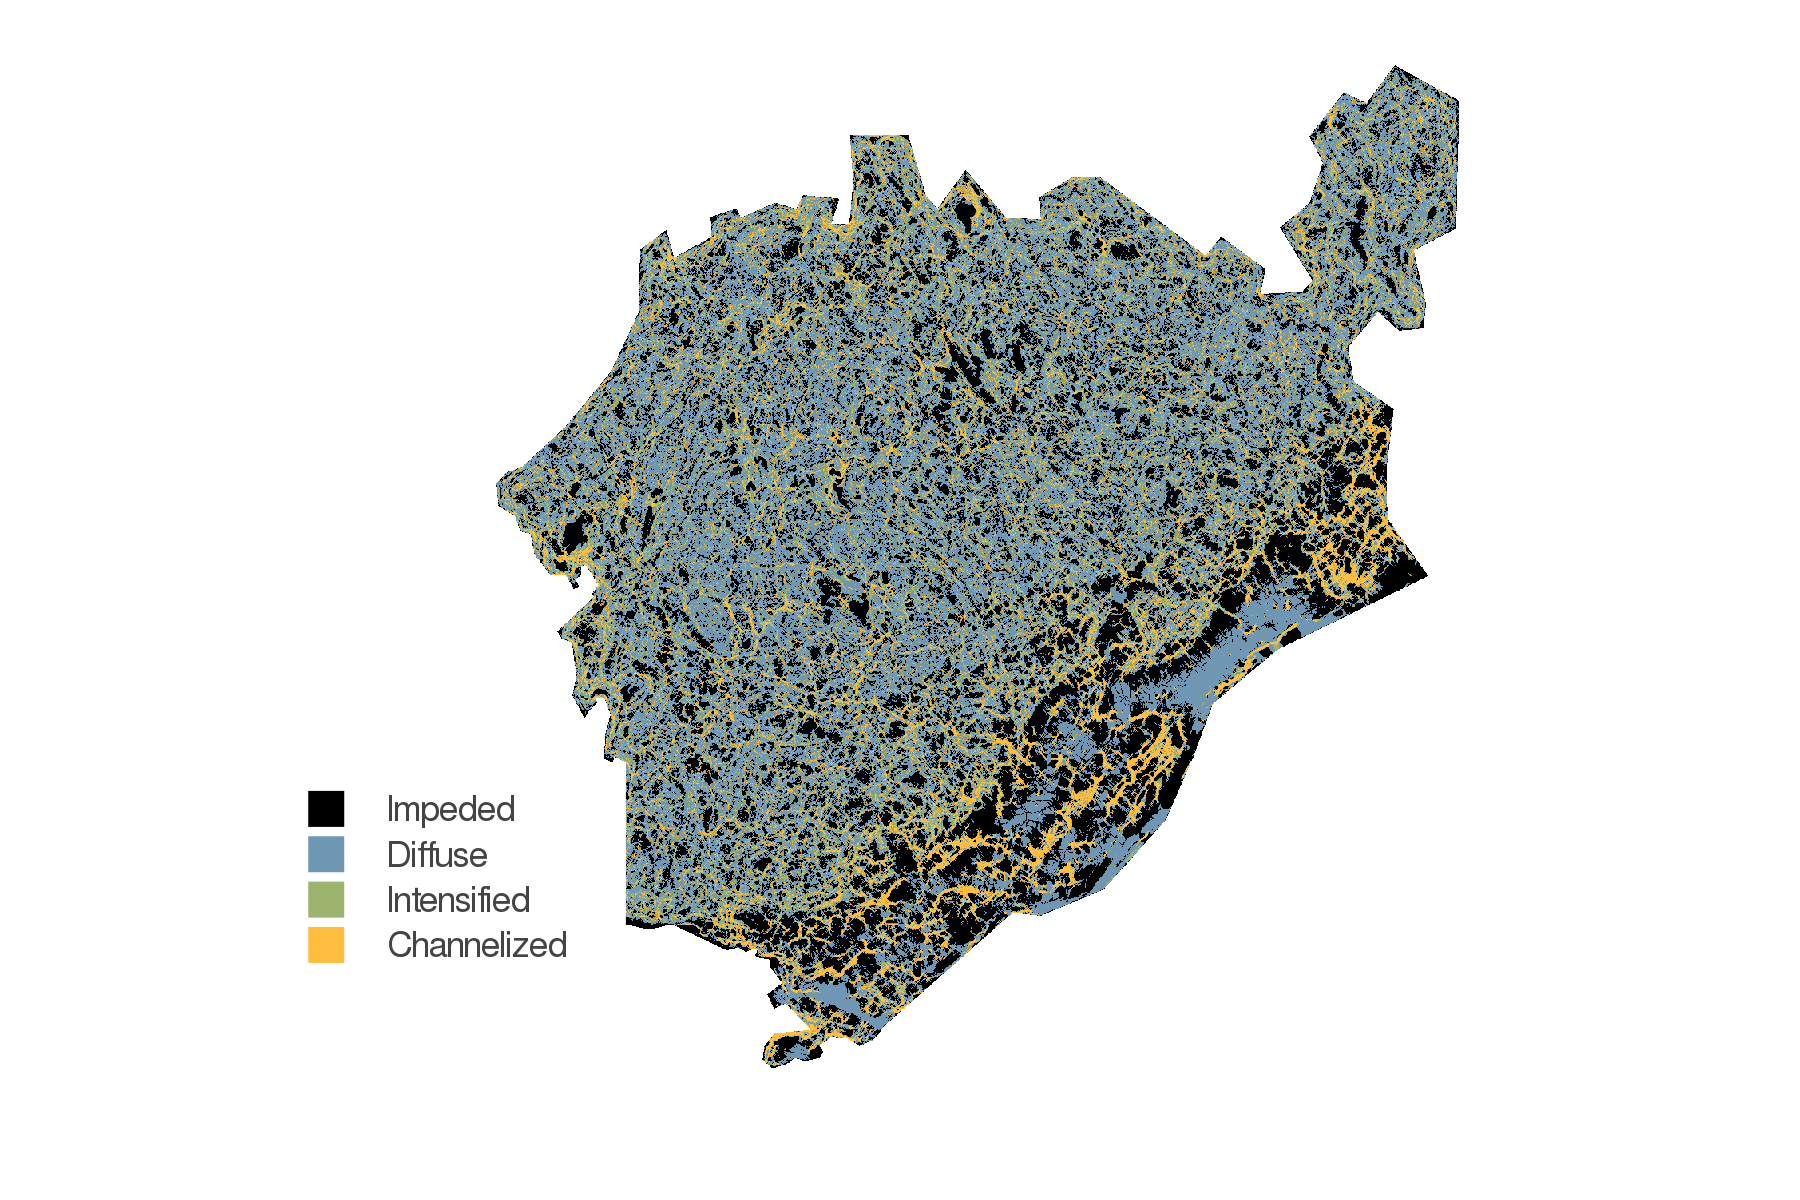
\includegraphics{figures/figure.png}
\caption{This is the legend of the figure, which will be shown in the
margin in preprint mode, and underneath the figure in draft mode. The
legend can contain references, etc. It is advised to use a resolution of
at least 600dpi for the figures.}\label{fig:figure}
}
\end{figure}

We can now use \texttt{@fig:figure} to refer to fig.~\ref{fig:figure}.

\hypertarget{example-text}{%
\section{Example text}\label{example-text}}

Connectance, defined as the ratio of realized interactions on the total
number of potential interactions, is one of the most common descriptor
of network structure. In a bipartite network with \(T\) species at the
top, and \(B\) at the bottom, having a total of \(L\) interactions, it
is defined as \(Co = L/(T\times B)\). Connectance has a lower bound, as
the network cannot have fewer interactions that the number of species in
its more speciose level -- the minimal connectance is therefore
\(c_m = \text{max}(T,B)\). This makes the connectance of networks of
different sizes difficult to compare, especially since bipartite
networks tends to have a low connectance. For this reason, we used a
corrected version of connectance, defined as

\begin{equation}\protect\hypertarget{eq:cstar}{}{Co^\star=\frac{L-c_m}{T\times B-c_m} \,.}\label{eq:cstar}\end{equation}

\hypertarget{this-is-a-subsection}{%
\subsection{This is a subsection}\label{this-is-a-subsection}}

This takes values between 0 (the network has the minimal number of
interactions) and 1 (all species are connected), but is robust to
variations in species richness.

\hypertarget{this-is-another-subsection}{%
\subsection{This is another
subsection}\label{this-is-another-subsection}}

This takes values between 0 (the network has the minimal number of
interactions) and 1 (all species are connected), but is robust to
variations in species richness.

\hypertarget{some-non-standard-maths}{%
\subsection{Some non-standard maths}\label{some-non-standard-maths}}

The phylogenetic reconstruction of \(\hat{\mathscr{L}}\) and
\(\hat{\mathscr{R}}\) has an associated uncertainty, represented by the
breadth of the uniform distribution associated to each of their entries.
Therefore, we can use this information to assemble a
\emph{probabilistic} metaweb in the sense of
(\textbf{Poisot2016StrPro?}), \emph{i.e.} in which every interaction is
represented as a single, independent, Bernoulli event of probability
\(p\).

Specifically, we have adopted the following approach. For every entry in
\(\hat{\mathscr{L}}\) and \(\hat{\mathscr{R}}\), we draw a value from
its distribution. This results in one instance of the possible left
(\(\hat{\mathscr{l}}\)) and right (\(\hat{\mathscr{r}}\)) subspaces for
the Canadian metaweb. These can be multiplied, to produce one matrix of
real values. Because the entries in \(\hat{\mathscr{l}}\) and
\(\hat{\mathscr{r}}\) are in the same space where \(\mathscr{L}\) and
\(\mathscr{R}\) were originally predicted, it follows that the threshold
\(\rho\) estimated for the European metaweb also applies. We use this
information to produce one random Canadian metaweb,
\(N = \hat{\mathscr{L}}\)\(\hat{\mathscr{R}}' \ge \rho\).

Because the intervals around some trait values can be broad (in fact,
probably broader than what they would actually be), we repeat the above
process \(2\times 10^5\) times, which results in a probabilistic metaweb
\(P\), where the probability of an interaction (here conveying our
degree of trust that it exists given the inferred trait distributions)
is given by the number of times where it appears across all random draws
\(N\), divided by the number of samples. An interaction with
\(P_{i,j} = 1\) means that these two species were predicted to interact
in all \(2\times 10^5\) random draws, etc..

\hypertarget{references}{%
\section*{References}\label{references}}
\addcontentsline{toc}{section}{References}

\hypertarget{refs}{}
\begin{CSLReferences}{1}{0}
\leavevmode\vadjust pre{\hypertarget{ref-Camerano1880EquViv}{}}%
Camerano, L. (1880). Dell'equilibrio dei viventi merce la reciproca
distruzione. \emph{Atti Della R. Accad. Delle Sci. Torino}, 15,
393--414.

\leavevmode\vadjust pre{\hypertarget{ref-Elton1927AniEco}{}}%
Elton, C.S. (1927). \emph{Animal ecology}. University of Chicago Press.

\end{CSLReferences}

\end{document}
